\section{FE--Meshfree mixed formulation with optimal constraint}

In the proposed mixed-formulation, the displacement is approximated using three-node, six-node triangular elements and four-node, eight-node quadrilateral elements \cite{hughes2000}. In order to flexcially adjust to let the dofs of pressure meets to be optimal, the reproducing kernel meshfree approximation is involved to approximate pressure.

\subsection{Reproducing kernel meshfree approximation}

In accordance with the reproducing kernel approximation, the entire domain $\Omega$ is discretized by $n_p$ meshfree points, $\{\boldsymbol x_I\}_{I=1}^{n_p}$. Each meshfree point equips a meshfree shape function $\Psi_I$ and nodal coefficient $p_I$, and the approximated pressure namely $p_h$ can be presented by:
\begin{equation}
p_h(\boldsymbol x) = \sum_{I=1}^{n_p} \Psi_I(\boldsymbol x) p_I
\end{equation}
where, in the reproducing kernel approximation framework, the shape function $\Psi_I$ is given by:
\begin{equation}\label{rkshape}
\Psi_I(\boldsymbol x) = \boldsymbol c(\boldsymbol x_I-\boldsymbol x) \boldsymbol p(\boldsymbol x_I-\boldsymbol x) \phi(\boldsymbol x_I - \boldsymbol x)
\end{equation}
in which $\boldsymbol p$ is the basis function, especially for 2D quadratic basis function, having the following form: 
\begin{equation}
\boldsymbol p(\boldsymbol x) = \{ 1, x, y, x^2, xy, y^2\}^T
\end{equation}
and $\phi$ stands for the kernel function. In this work, the traditional Cubic B-spline function with square suppot is used as the kernel function:
\begin{equation}
\phi(\boldsymbol x_I-\boldsymbol x) = \phi(s_x) \phi(s_y), \quad s_i = \frac{\Vert \boldsymbol x_I - \boldsymbol x\Vert}{\bar s_{iI}}
\end{equation}
with
\begin{equation}
\phi(s) =\frac{1}{3!} \begin{cases}
    (2-2s)^3 - 4(1-2s)^3 & s\le\frac{1}{2} \\
    (2-2s)^3 &\frac{1}{2}<s<1 \\
    0 & s> 1
\end{cases}
\end{equation}
where $\bar s_{iI}$'s are the support size towards the $i$-direction for the shape function $\Psi_I$.
The correction function $\boldsymbol c$ can be determined by the following so-call consistency condition:
\begin{equation}\label{cc1}
\sum_{I=1}^{n_p}\Psi_I(\boldsymbol x) \boldsymbol p(\boldsymbol x_I) = \boldsymbol p (\boldsymbol x)
\end{equation}
or equivalent shifted form:
\begin{equation}\label{cc2}
\sum_{I=1}^{n_p}\Psi_I(\boldsymbol x) \boldsymbol p(\boldsymbol x_I-\boldsymbol x) = \boldsymbol p (\boldsymbol 0)
\end{equation}
Substituting Eq. \ref{rkshape} into Eq. \eqref{cc2} leads to:
\begin{equation}\label{correction}
\boldsymbol c(\boldsymbol x_I-\boldsymbol x) = \boldsymbol A^{-1}(\boldsymbol x_I-\boldsymbol x)\boldsymbol p(\boldsymbol 0)
\end{equation}
in which $\boldsymbol A$ is namely moment matrix evaluating by:
\begin{equation}
\boldsymbol A(\boldsymbol x_I-\boldsymbol x) = \sum_{I=1}^{n_p}\boldsymbol p(\boldsymbol x_I-\boldsymbol x) \boldsymbol p^T(\boldsymbol x_I-\boldsymbol x)\phi(\boldsymbol x_I-\boldsymbol x)
\end{equation}
Taking Eq. \eqref{correction} back to Eq. \eqref{rkshape}, the final form of reproducing kernel shape function can be got as:
\begin{equation}
\Psi_I(\boldsymbol x) = \boldsymbol p^T(\boldsymbol 0) \boldsymbol A^{-1}(\boldsymbol x_I-\boldsymbol x)\phi(\boldsymbol x_I-\boldsymbol x)
\end{equation}

% discuss of advantages

\subsection{Optimal pressure nodes distributions}

In this subsection, the FE-meshfree mixed formulation is empolyed in inf--sup test \cite{chapelle1993} to validate the proposed estimator of inf--sup value.
Consider the square domain $\Omega = (0,1)\otimes (0,1)$ in Fig. \ref{fg:inf_sup_test},
the displacement is discretized by linear Triangular element (Tri3), Quadrilateral element (Quad4) with
$4\times 4$, $8\times 8$, $16\times 16$ and $32\times 32$ elements,
quadratic Triangular element (Tri6), Quadrilateral element (Quad8) with 
$2\times 2$, $4\times 4$, $8\times 8$ and $16\times 16$ elements, respectively.
In order to avoid the influence of interpolation error,
the uniform nodal distributions are used for pressure discretizations.

\begin{figure}[H]
\centering

\includegraphics[width=0.5\textwidth]{png/infsup_model.png}
\caption{Illustration of inf--sup test}\label{fg:inf_sup_test}
\end{figure}

Figure \ref{fg:infsup_convergence} shows the corresponding results, in which the red line stands for the value of $\beta$ respected to the number of pressure nodes $n_p$, the vertical dash line denotes to the stabilized number $n_s$.
The deeper color of lines means the mesh refining.
The results show that,
no matter linear or quadratic elements, as $n_p$ increases over the $n_s$, the $beta$'s value sharply decrease, and then the inf--sup condition cannot be maintained.
This result is consistent with the discussion in Section \ref{sec:constraint_ratio},
and again verify the effect of the proposed estimator.

\begin{figure}[H]
\centering
\begin{subcaptiongroup}
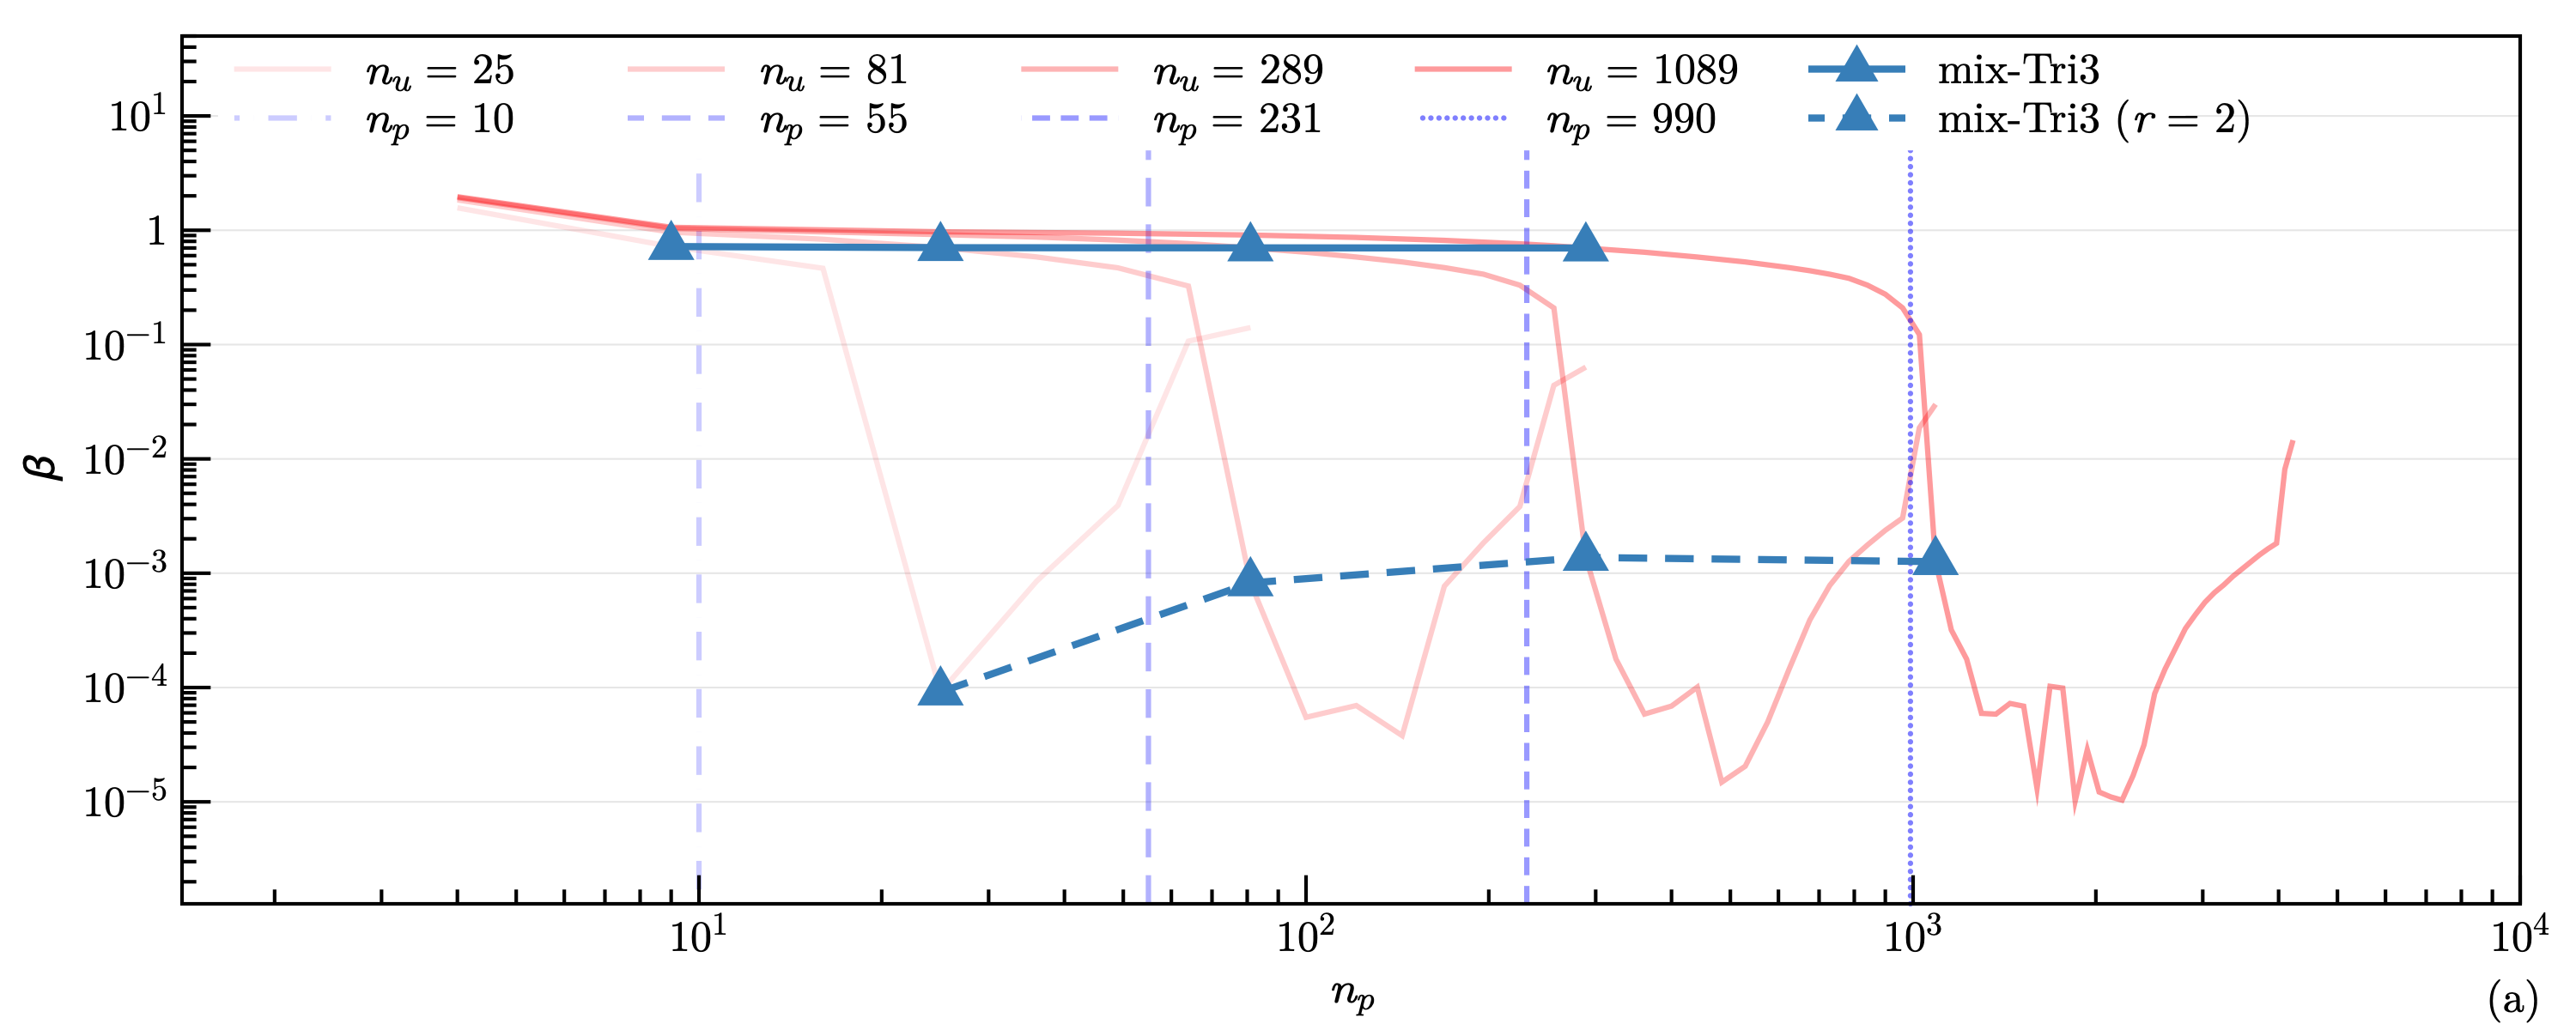
\includegraphics[width=\textwidth]{png/infsup_tri3.png}\phantomcaption\label{a}
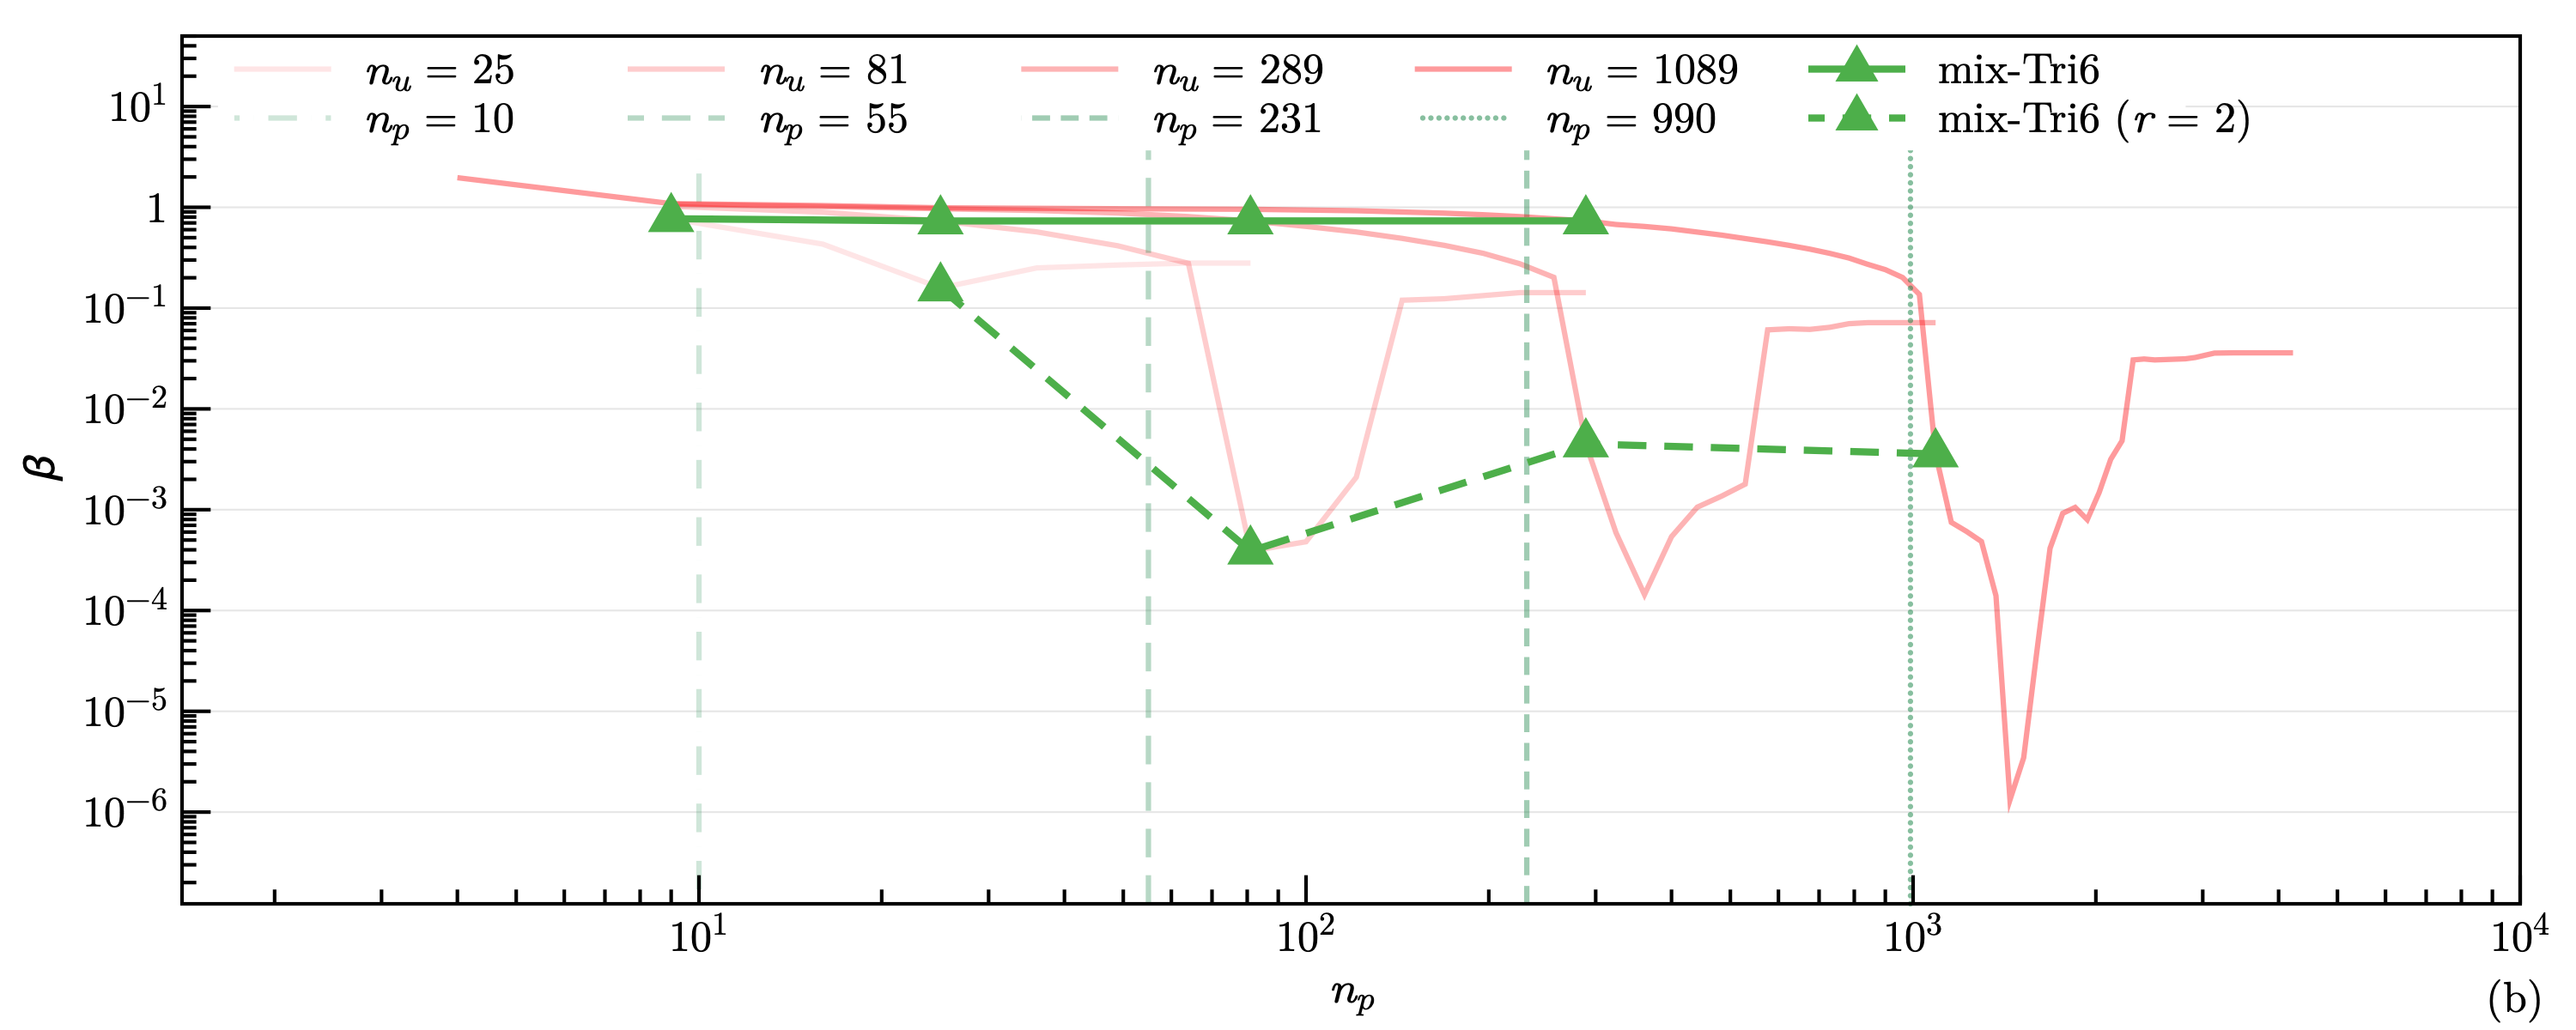
\includegraphics[width=\textwidth]{png/infsup_tri6.png}\phantomcaption\label{b}
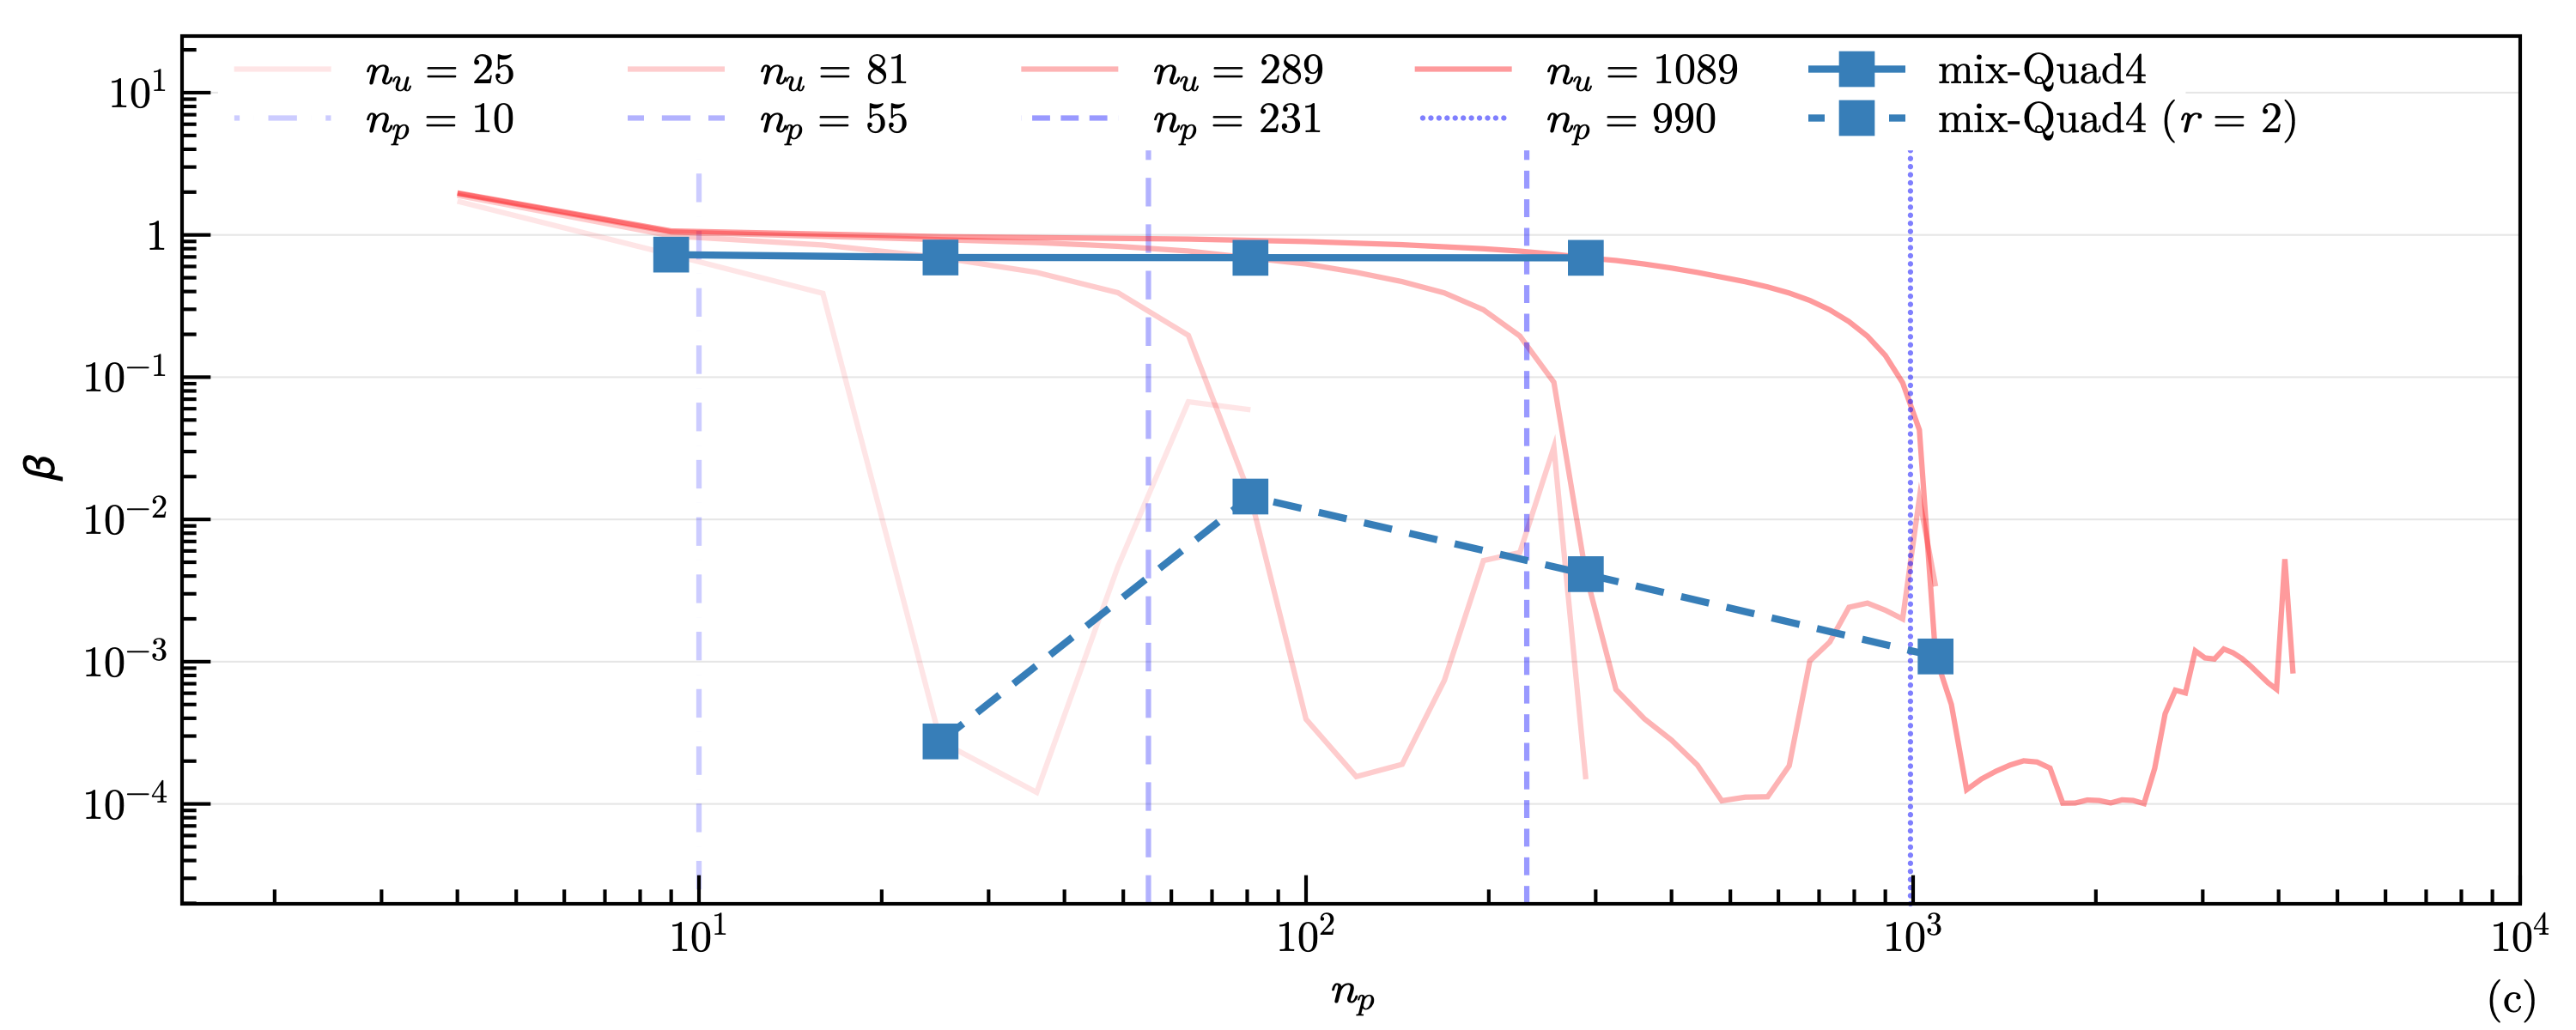
\includegraphics[width=\textwidth]{png/infsup_quad.png}\phantomcaption\label{c}
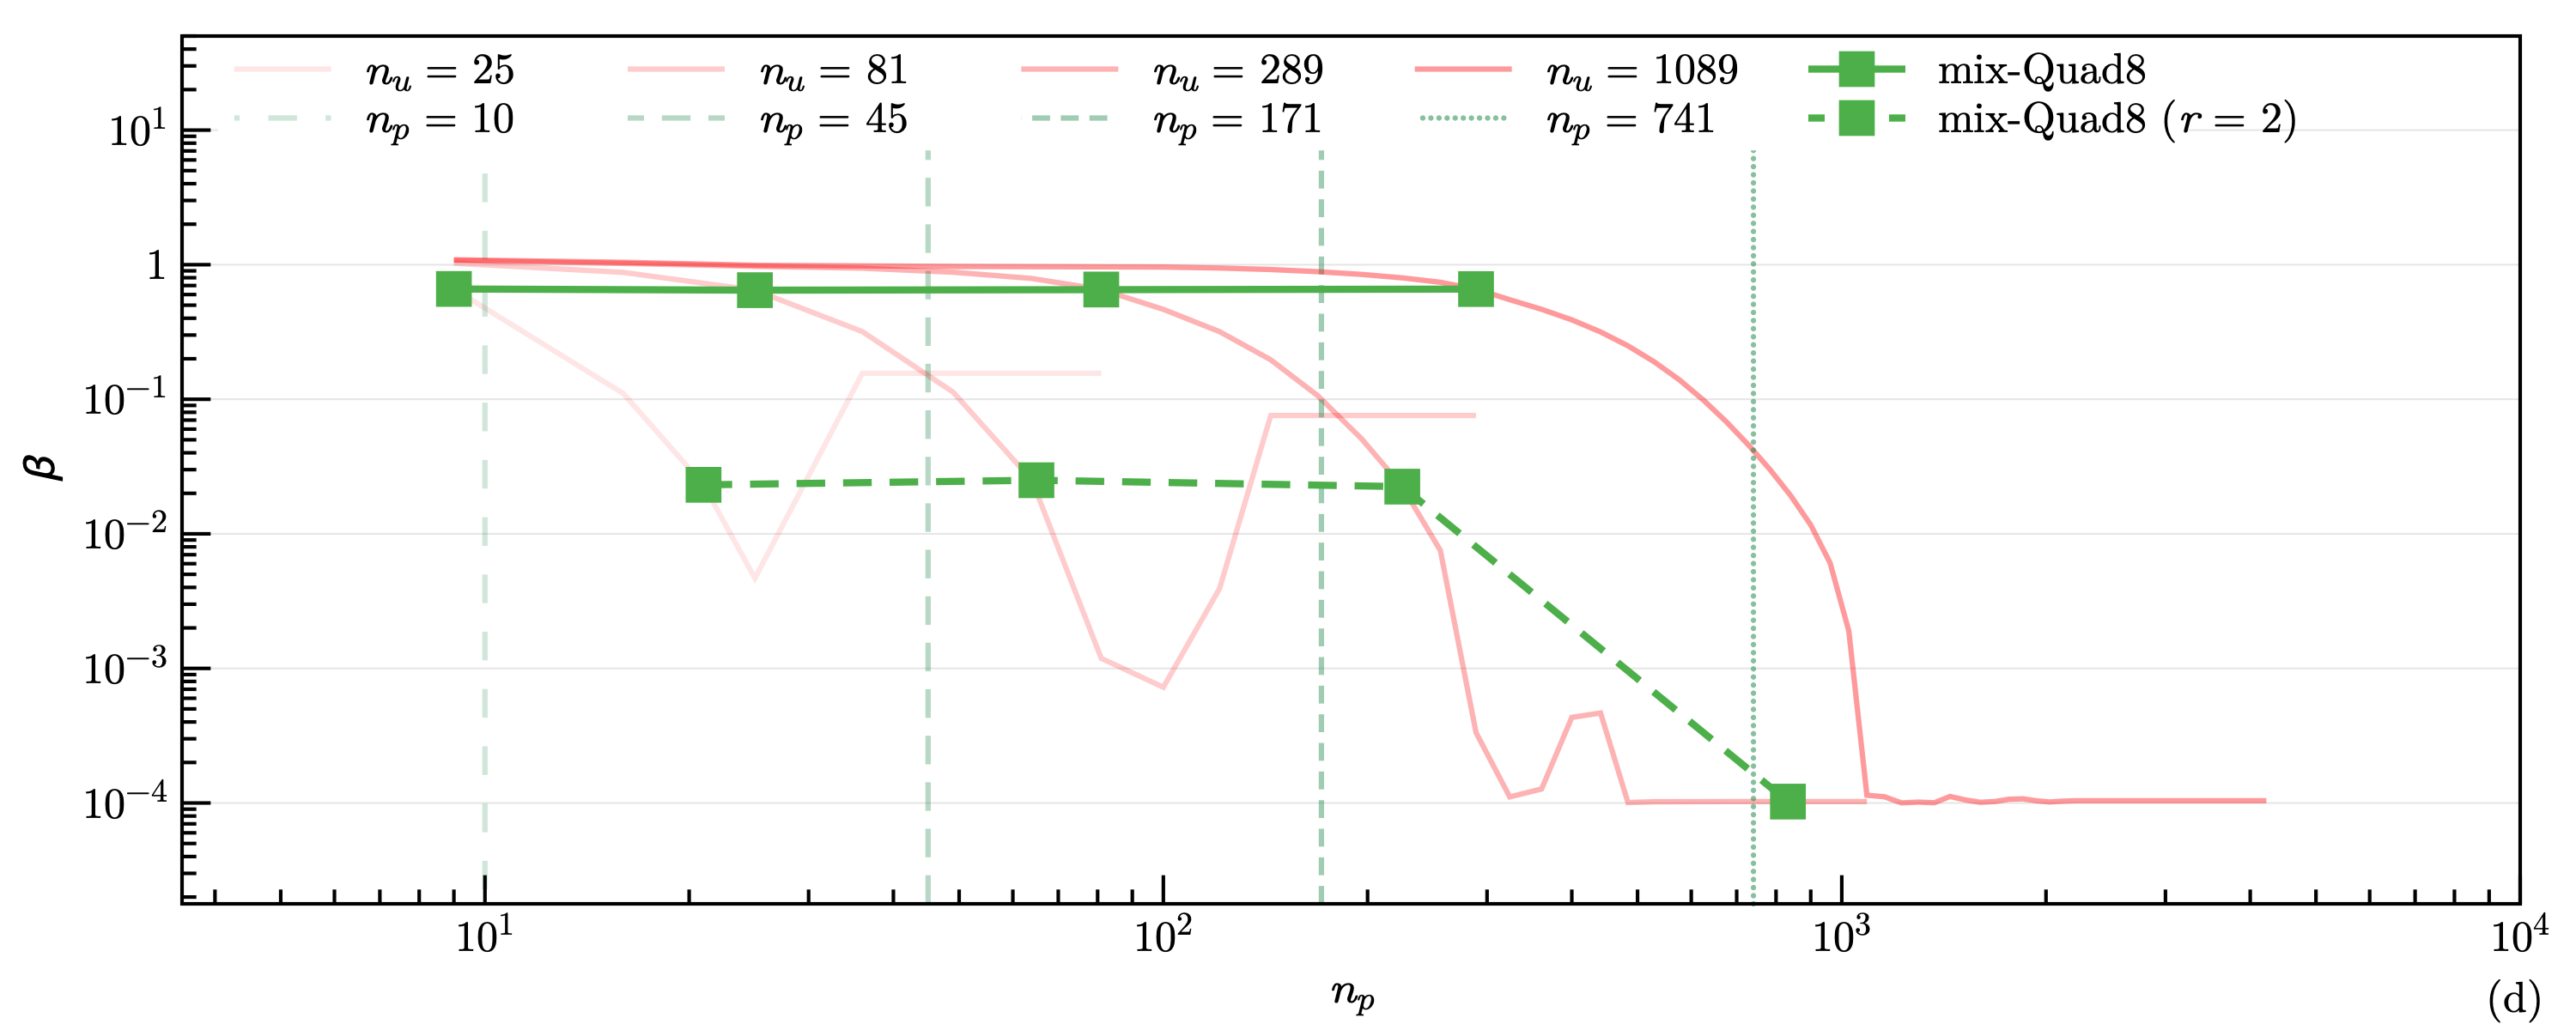
\includegraphics[width=\textwidth]{png/infsup_quad8.png}\phantomcaption\label{d}
\end{subcaptiongroup}
\captionsetup{aboveskip=0pt}
\caption{\centering Inf--sup test for various finite element formulations: \\ (\subref{a}) mix-Tri3; (\subref{b}) mix-Tri6; (\subref{c}) mix-Quad4; (\subref{d}) mix-Quad8}
\label{fg:infsup_convergence}
\end{figure}

Moreover, the mixed formulation's results with traditional optimal constraint ratio $r=n_d$ are listed in \ref{fg:infsup_convergence} as well,
and the $beta$ in this circumstance is already much smaller than those in optimal range.
Considering the results shown above, the easy-programming and efficiency,
the pressure nodes are chosen among the displacement nodes.
The final schemes for linear and quadratic, 2D and 3D elements discretizations are shown in Figure \ref{fg:mix_scheme},
in which all constraint ratios are belong to the range of optimal ratio.
The corresponding inf--sup test results for these schemes also be marked in Figure \ref{fg:inf_sup_test} and show that,
with the mesh refining, their $beta$'s are always maintained in a non--negligible level.

\begin{figure}[H]
    \centering
    \begin{tabular}{c@{\hspace{24pt}}c}
        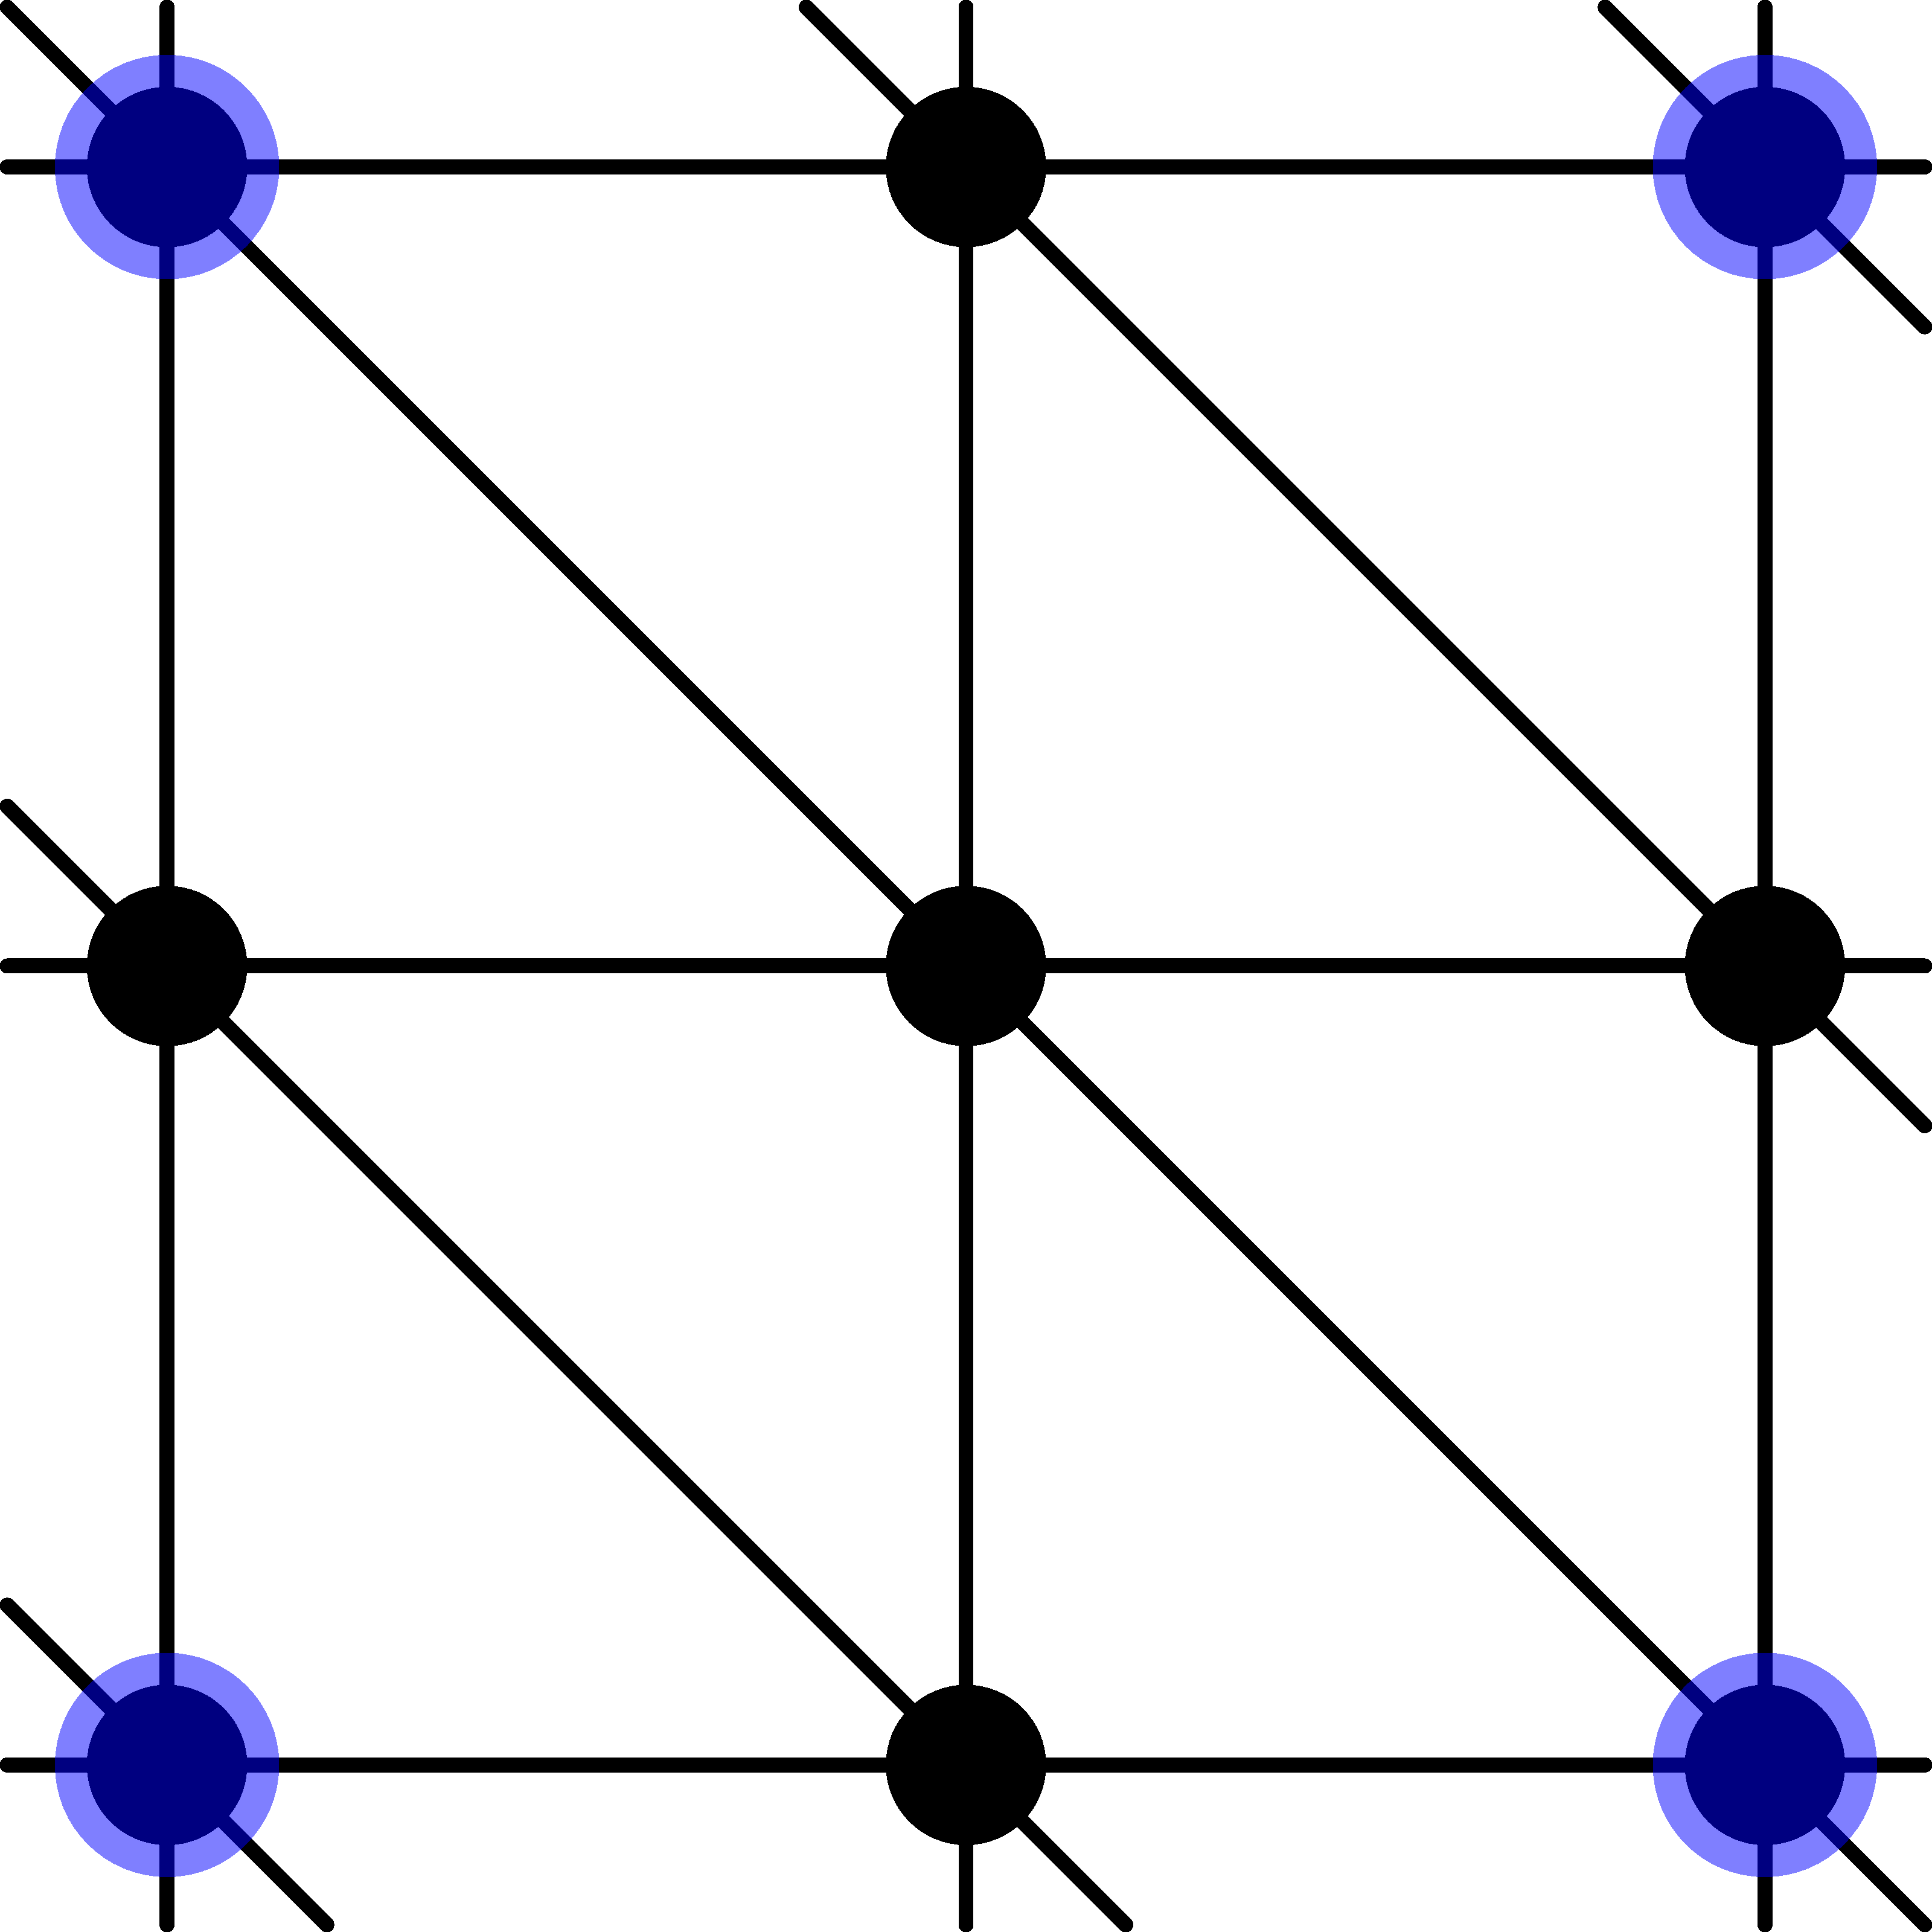
\includegraphics[width=0.3\textwidth]{png/mix_tri3.png} &
        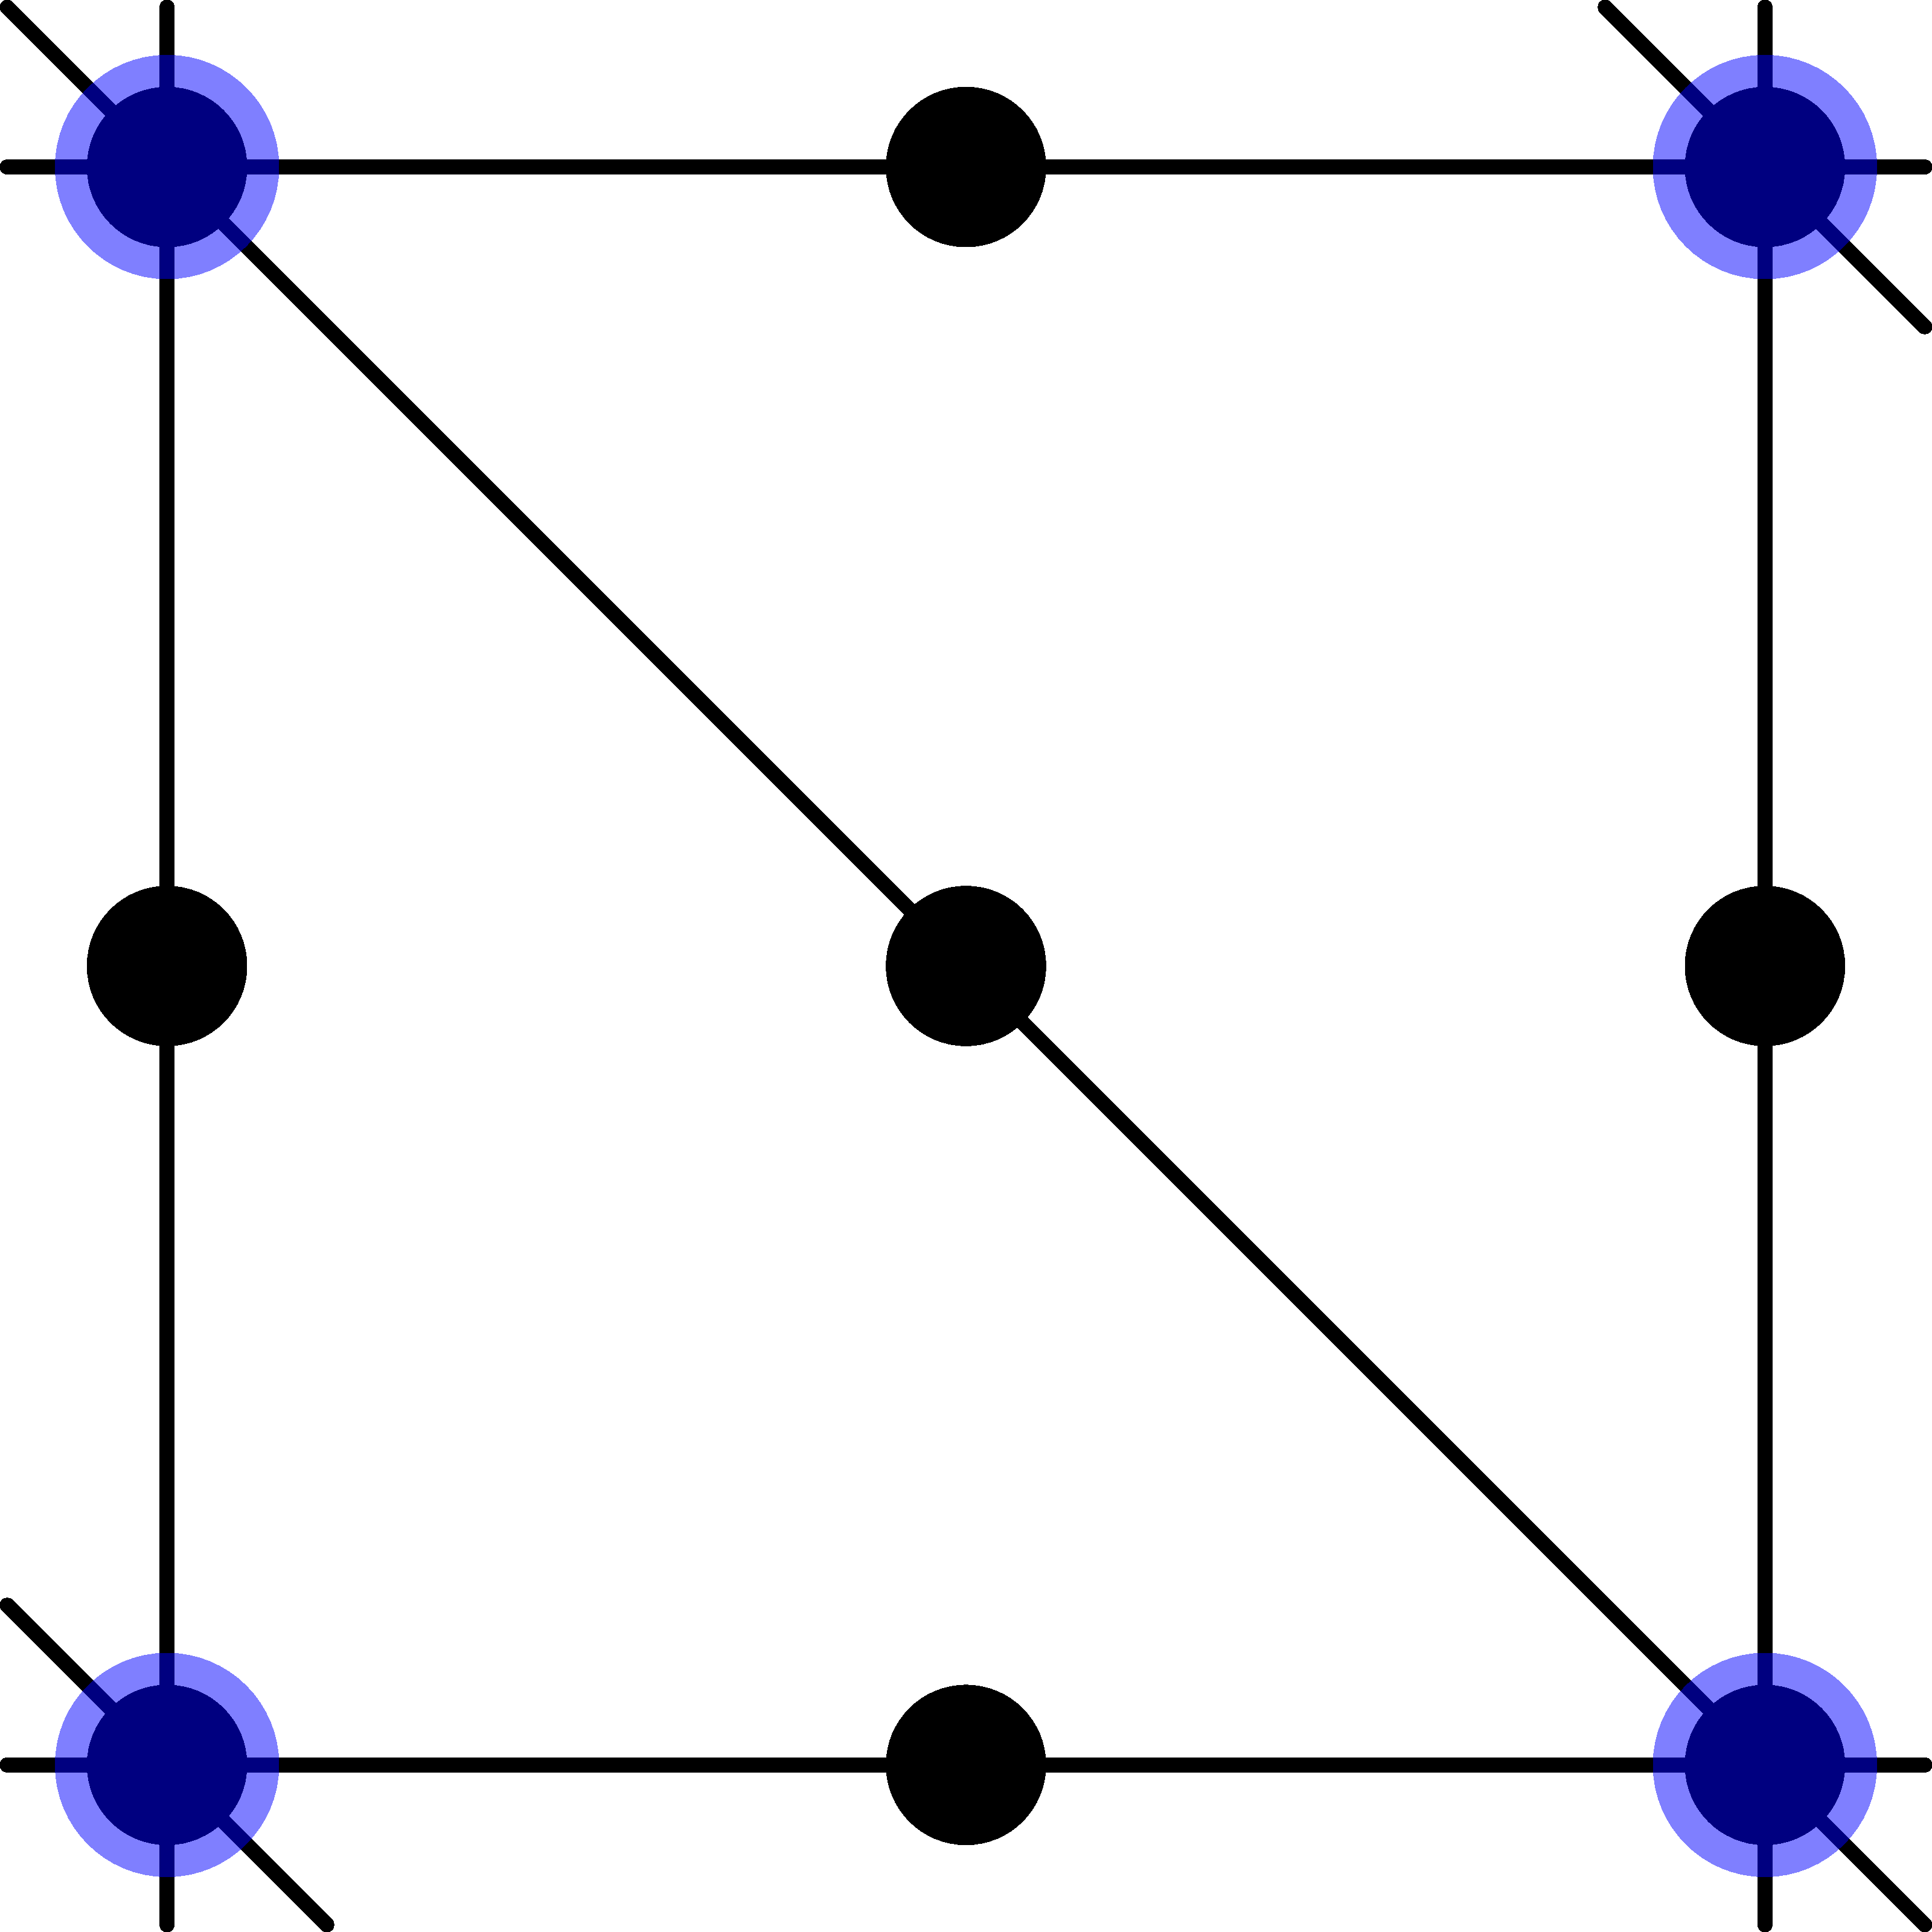
\includegraphics[width=0.3\textwidth]{png/mix_tri6.png} \\
        mix--Tri3 & mix--Tri6 \\
        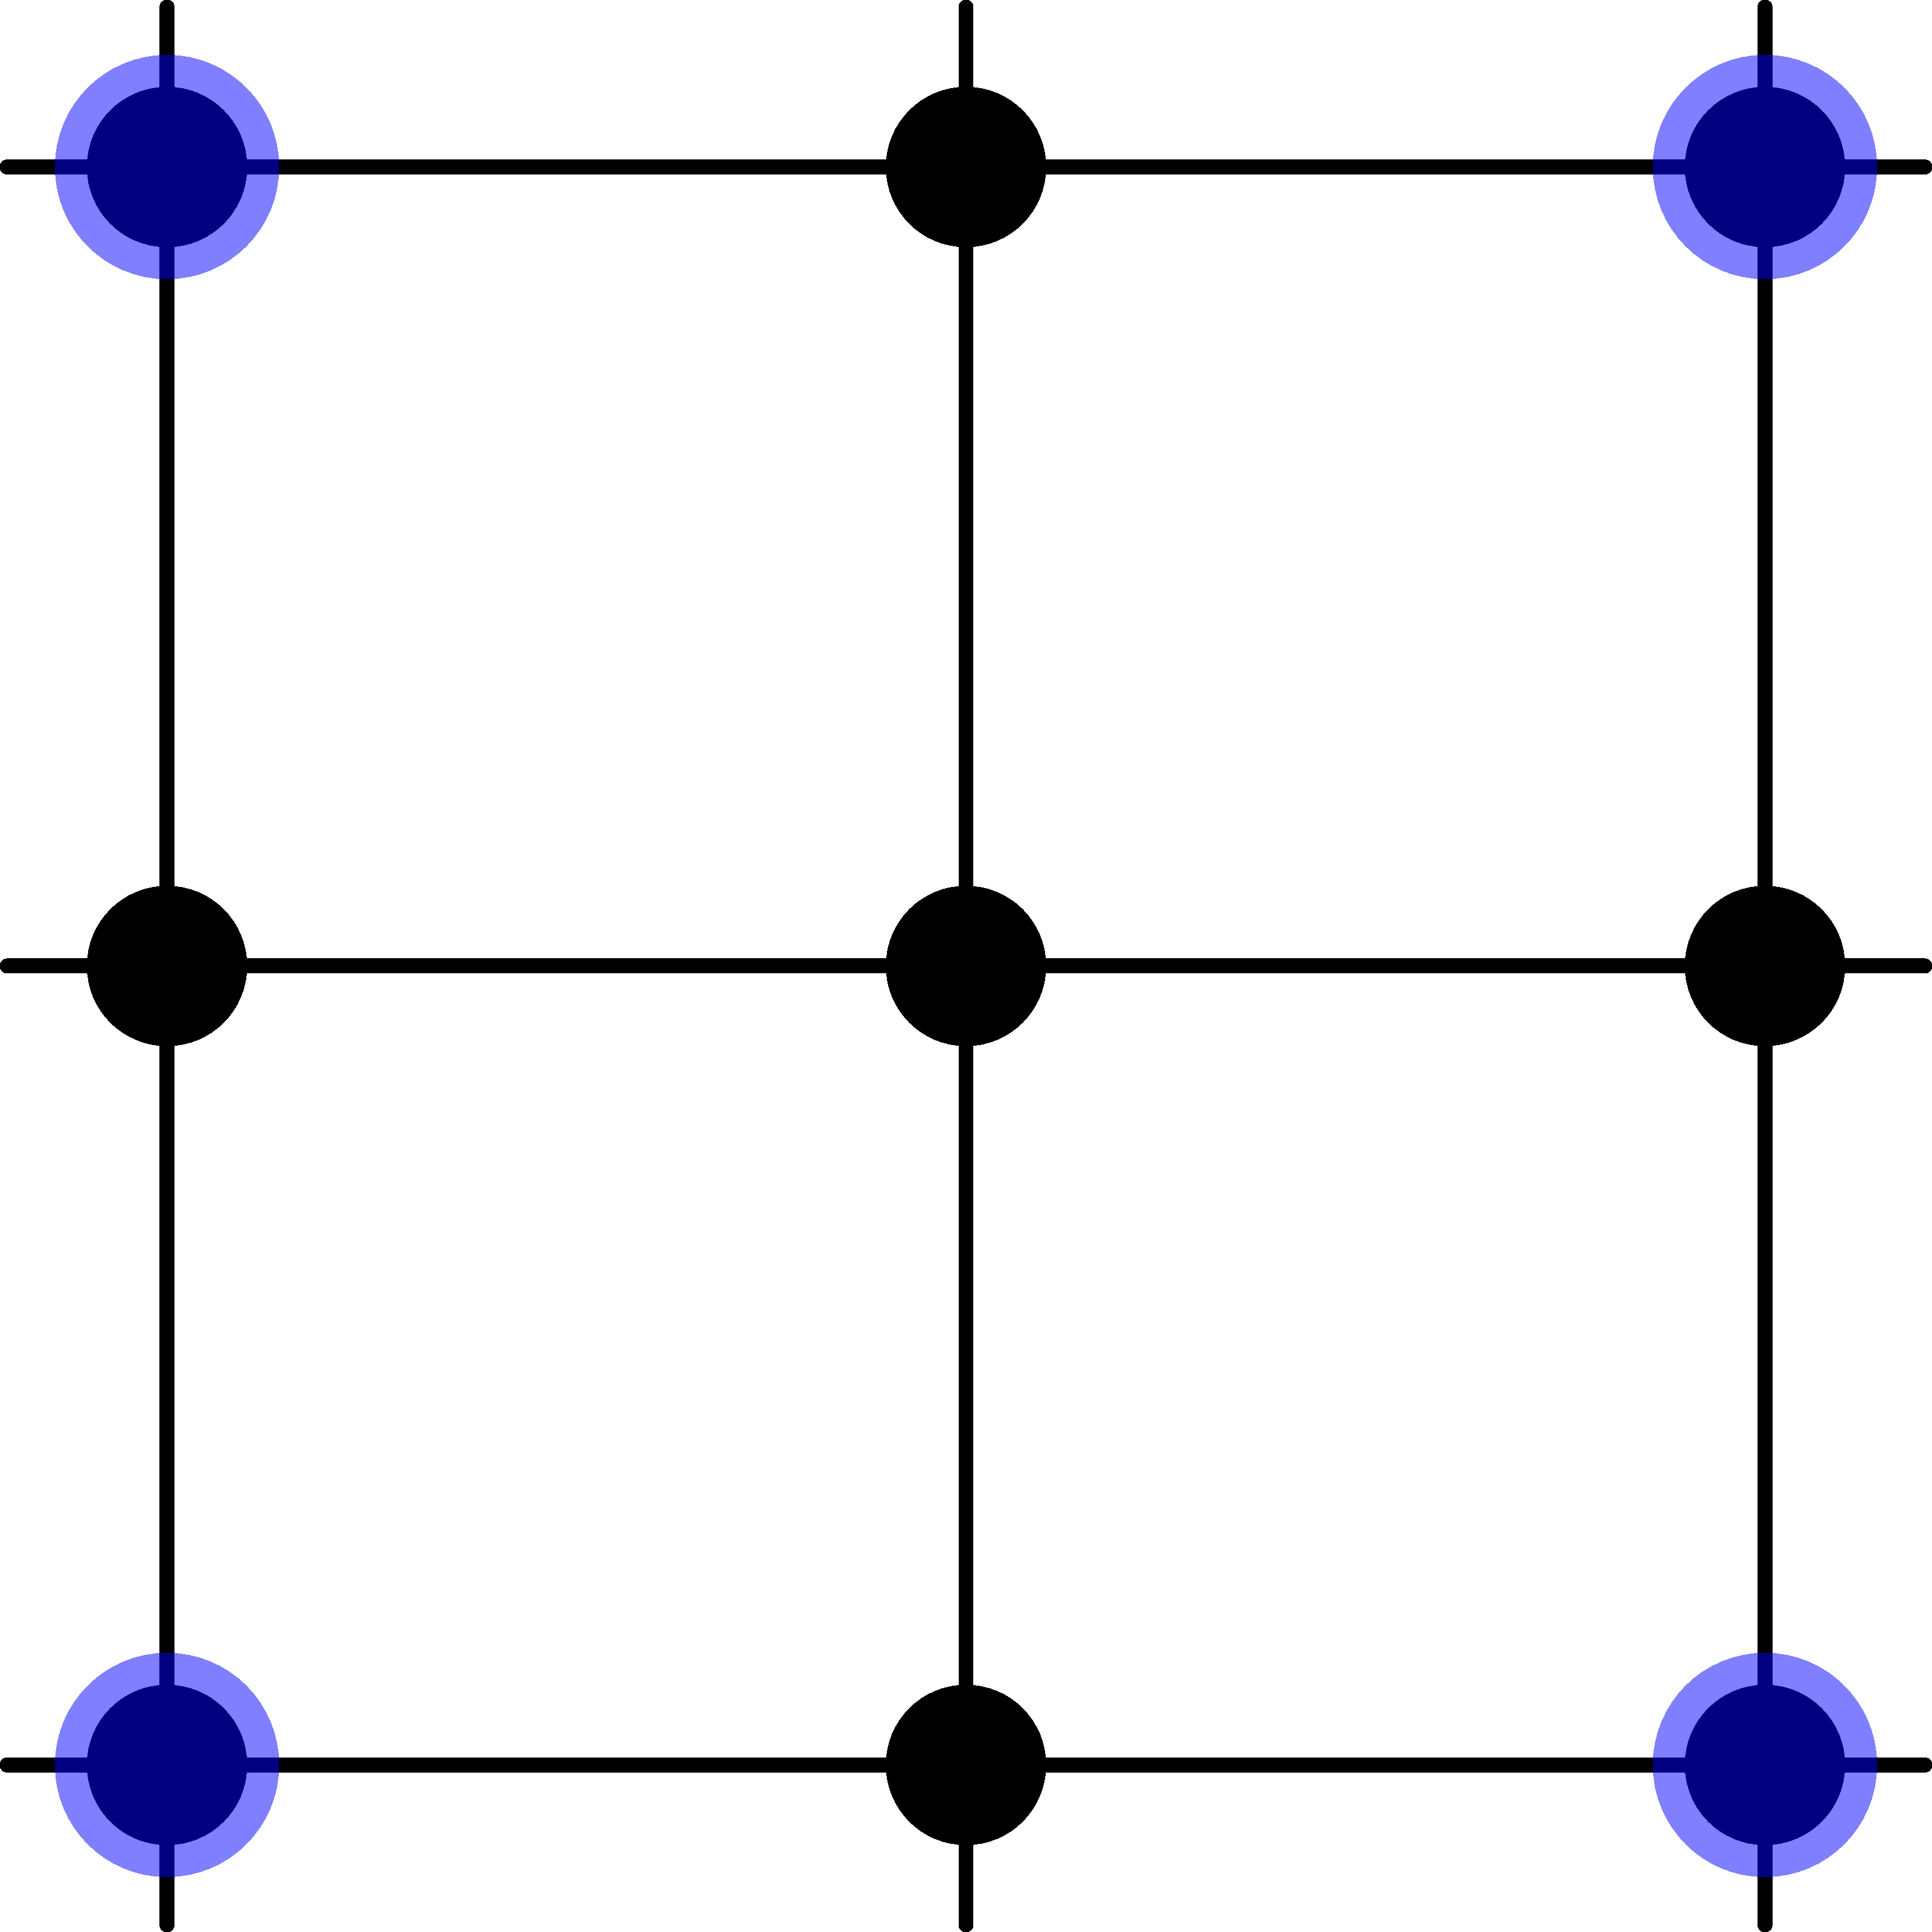
\includegraphics[width=0.3\textwidth]{png/mix_quad4.png} &
        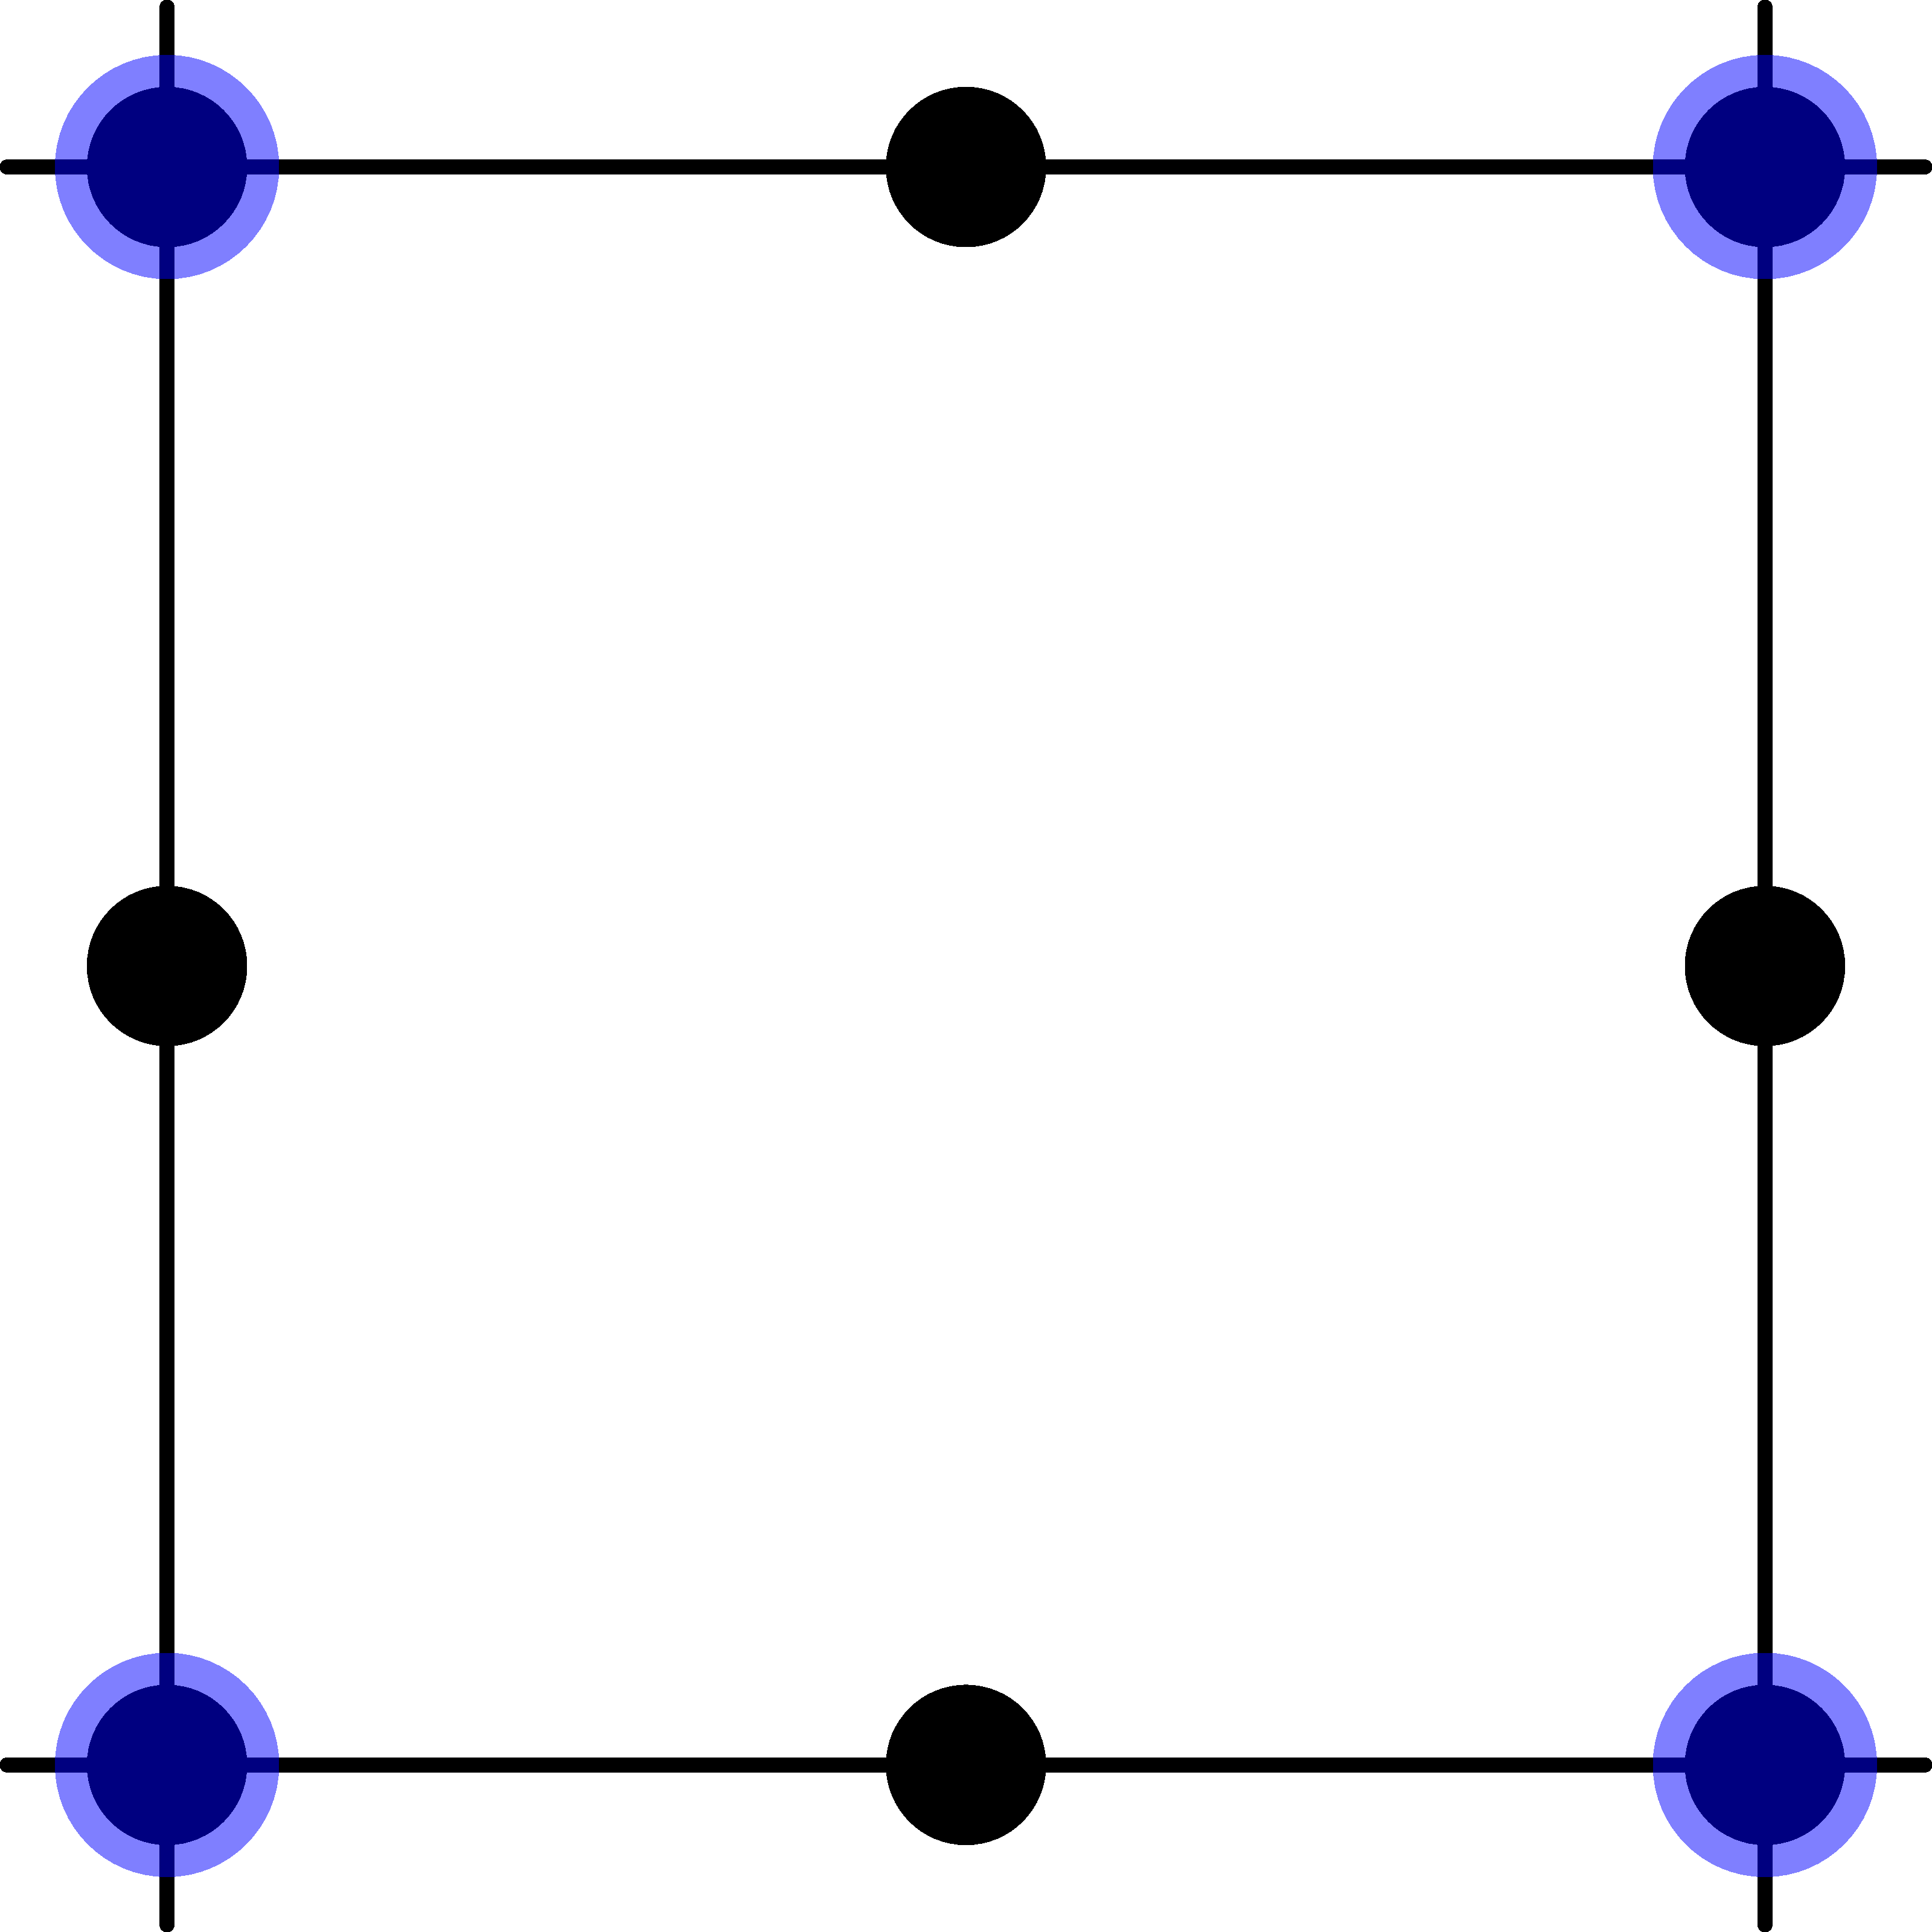
\includegraphics[width=0.3\textwidth]{png/mix_quad8.png} \\
        mix--Quad4 & mix--Quad8 \\
        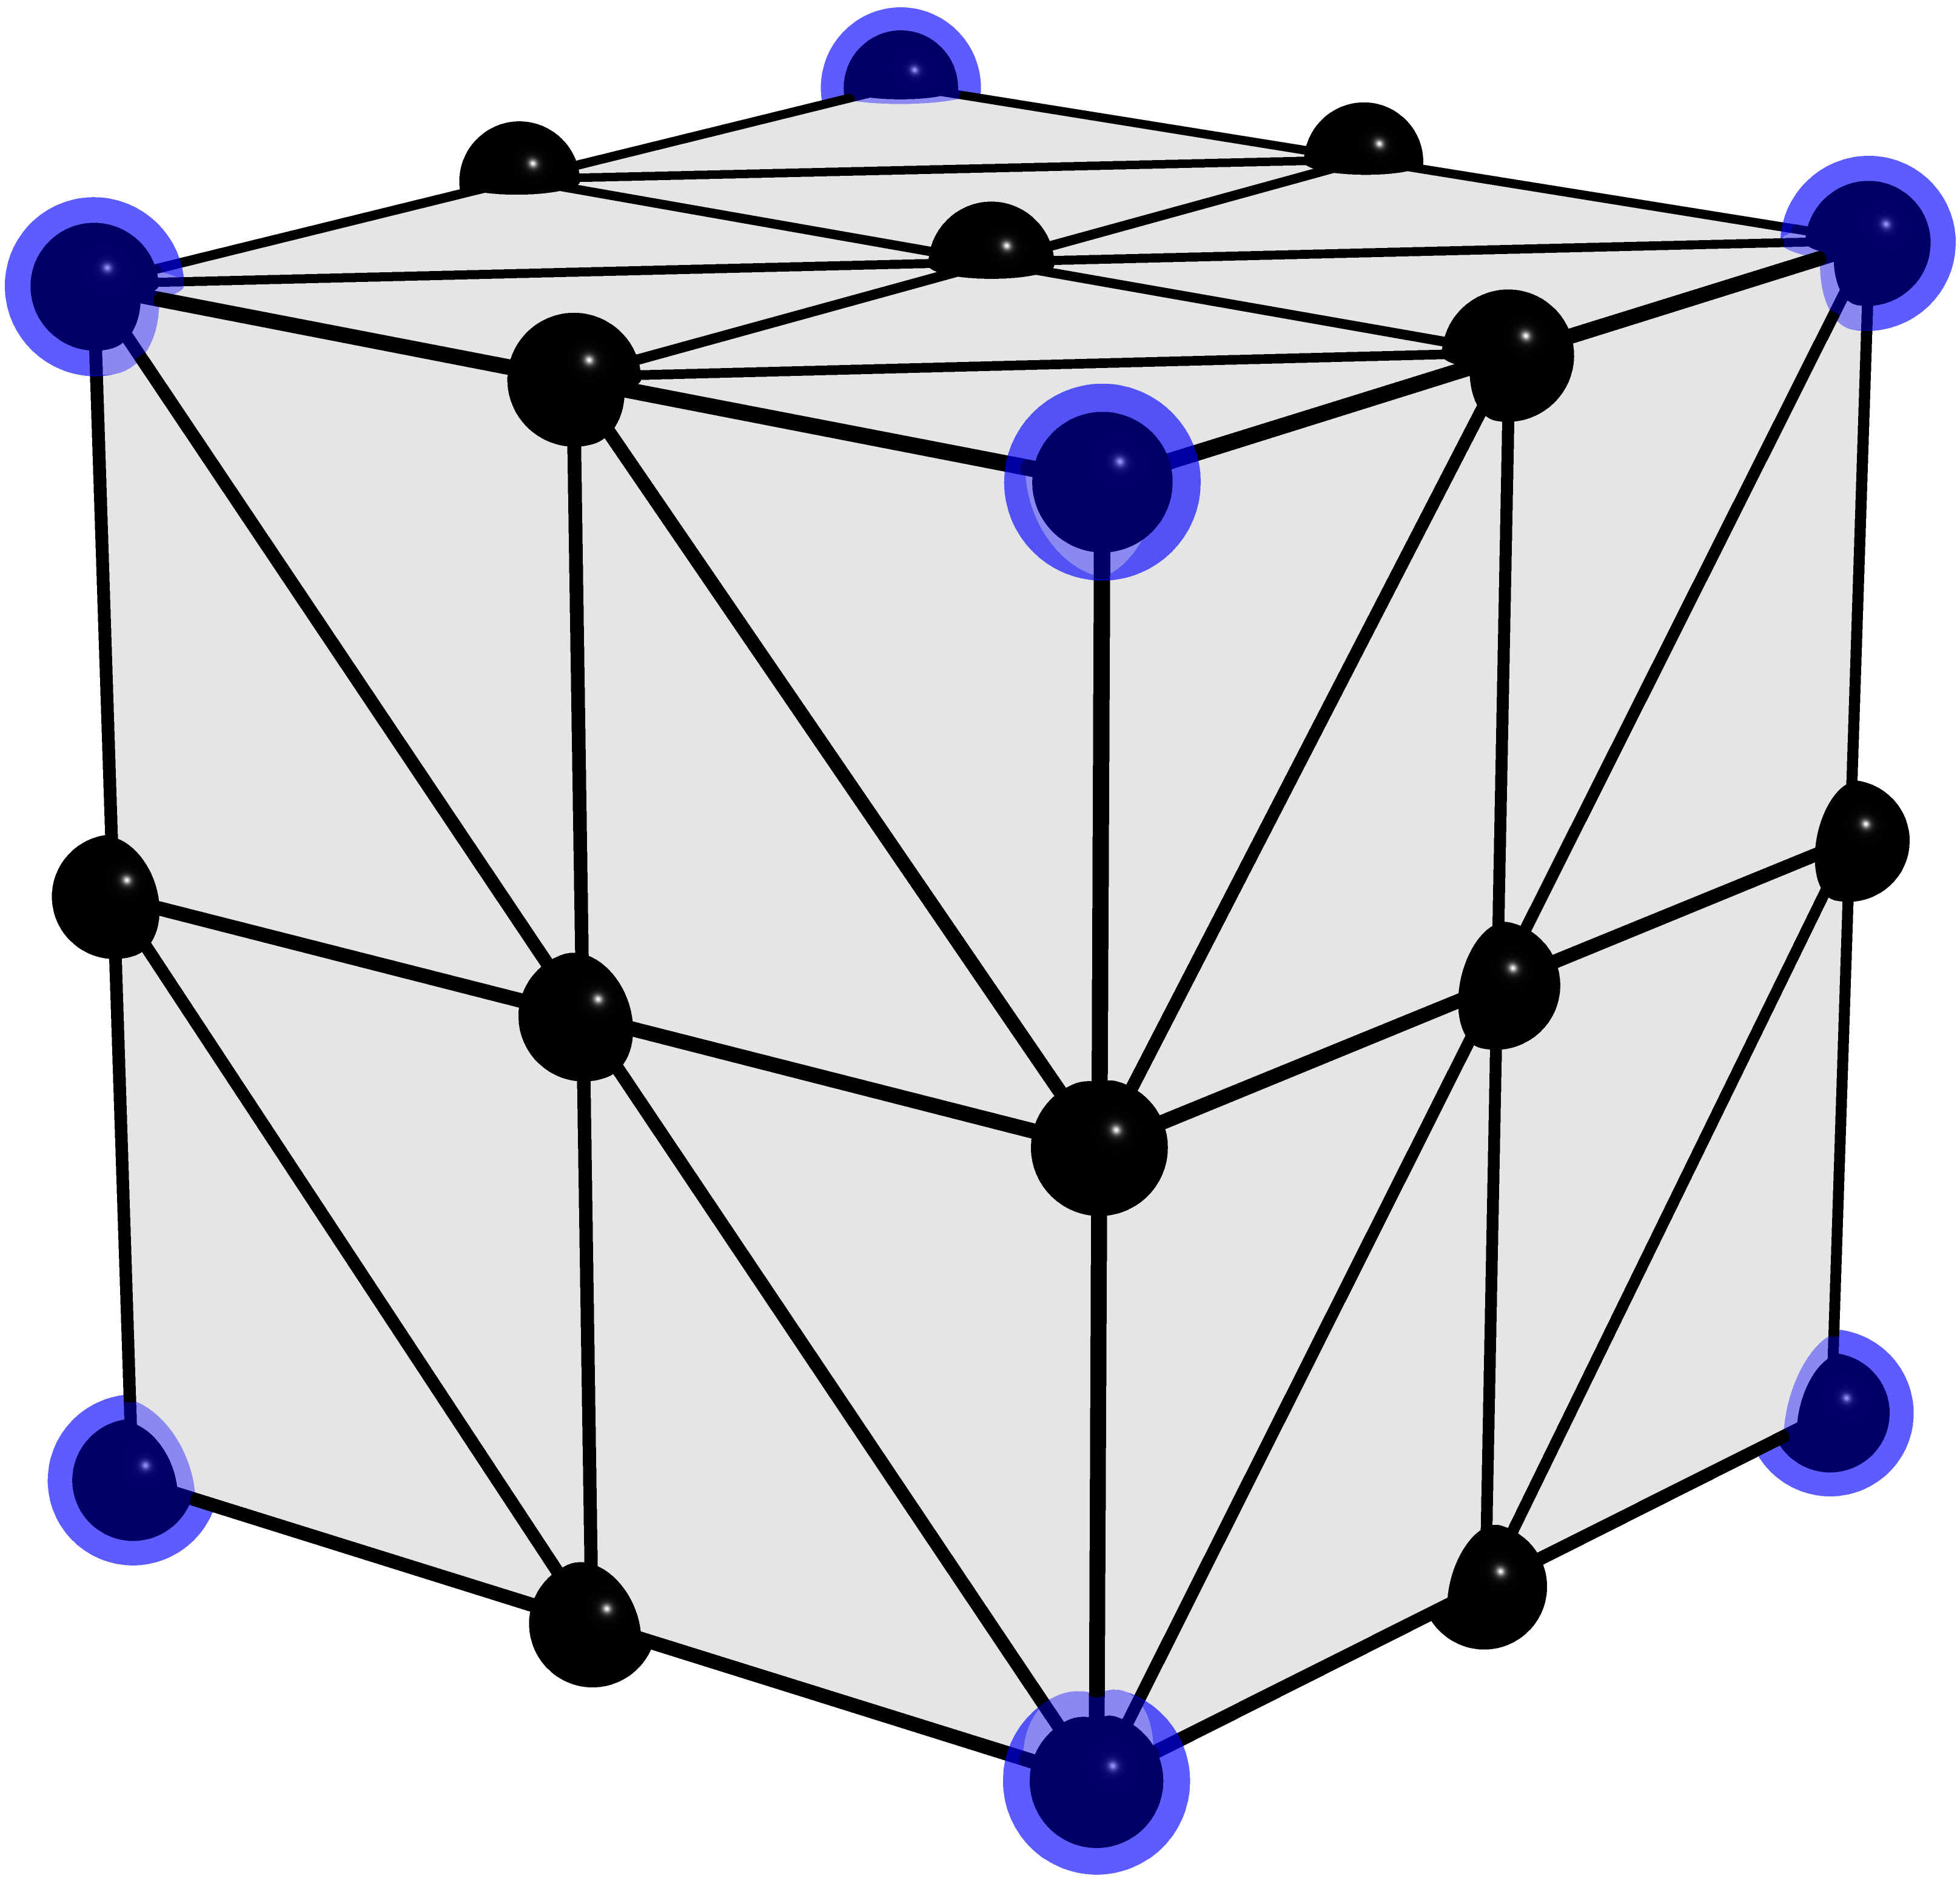
\includegraphics[width=0.3\textwidth]{png/mix_tet4.png} &
        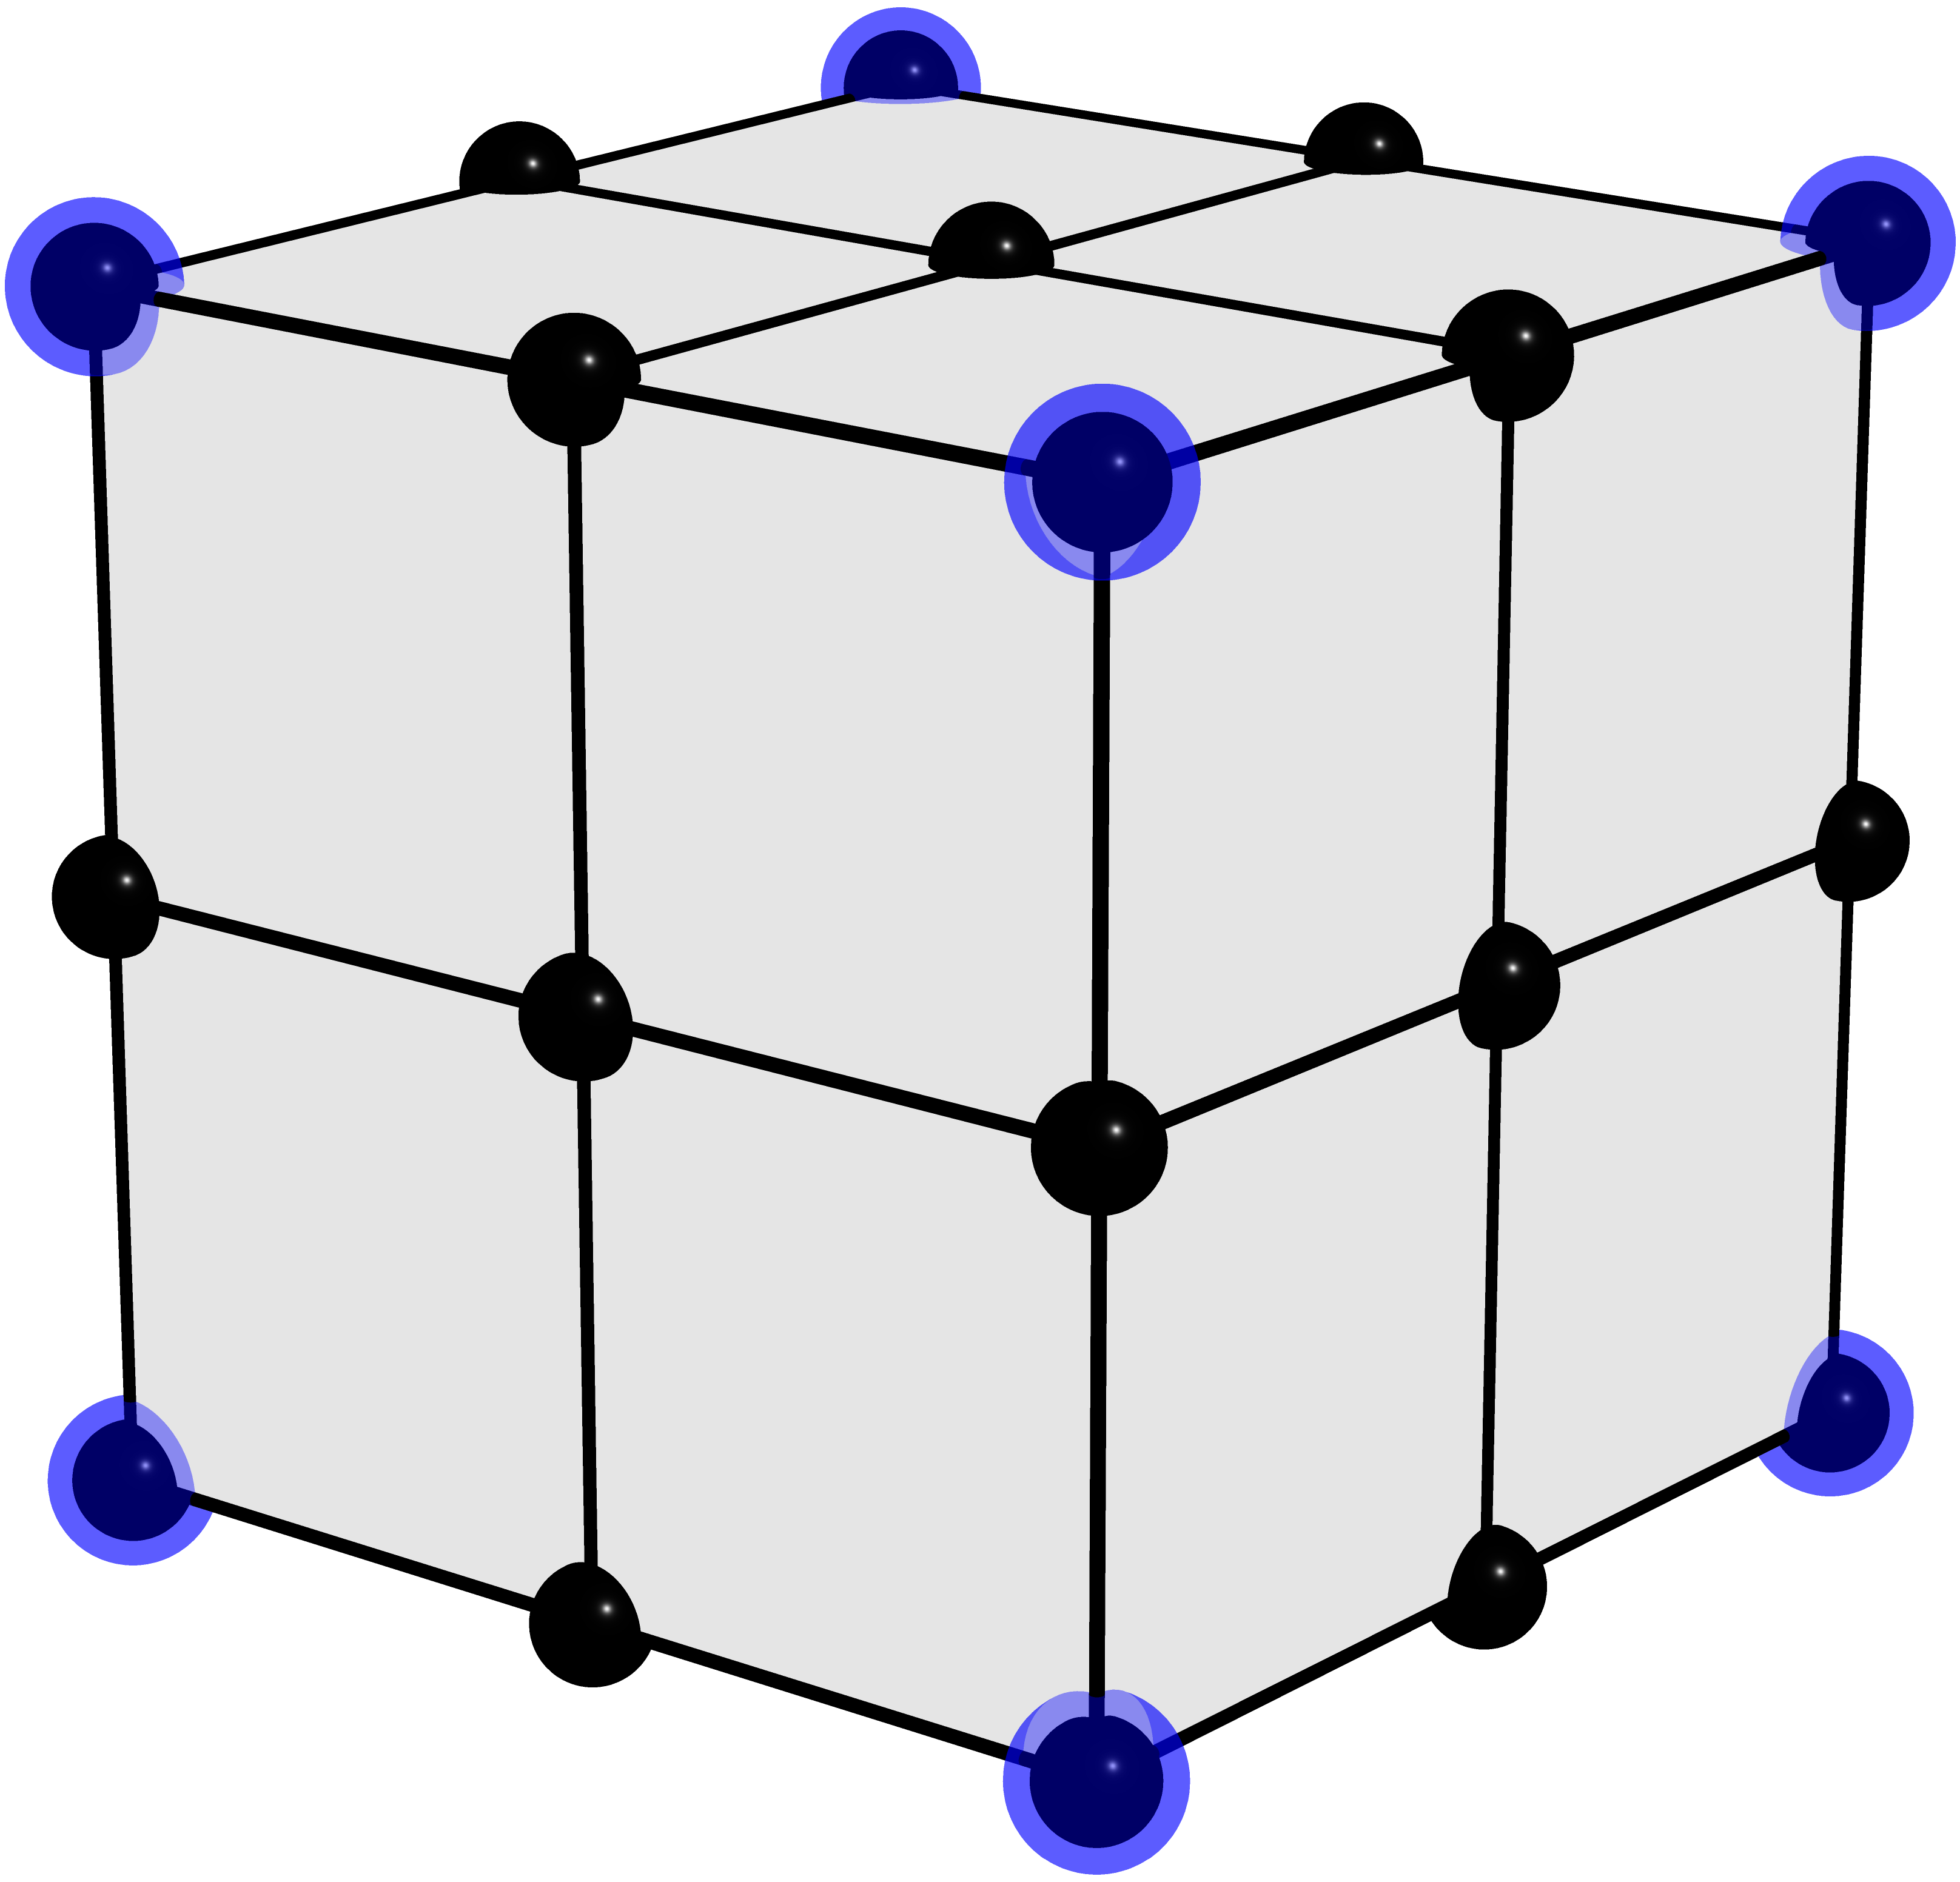
\includegraphics[width=0.3\textwidth]{png/mix_hex8.png} \\
        mix--Tet4 & mix--Hex8 \\
        \raisebox{-0.3\height}{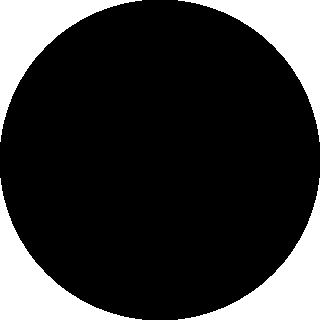
\includegraphics[width=12pt]{png/legend_u.png}} Displacement node: &
        \raisebox{-0.3\height}{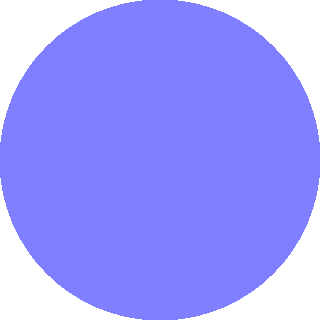
\includegraphics[width=12pt]{png/legend_p.png}} Pressure node:
    \end{tabular}
    \caption{Nodal distribution schemes for FE-MF mixed formulations with $r = r_{opt}$}\label{fg:mix_scheme}
\end{figure}

